\definecolor{tiffanyblue}{RGB}{129,216,208}
\definecolor{bangdiblue}{RGB}{0,149,182}
\definecolor{kleinblue}{RGB}{0,47,167}
\definecolor{kabuliblue}{RGB}{26,85,153}
\definecolor{purple}{RGB}{138,43,226}
\usetikzlibrary{matrix}
% \usetikzlibrary{external}
%----------------------------------------------
\begin{figure}[tbhp]
\vspace{-0.1in}
  \centering
\subfigure[Head Distance vs Encoder Depth] { \label{fig:visiualization_head_distance} 
    \centering
  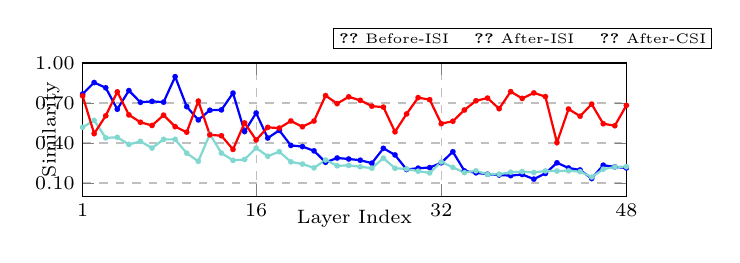
\begin{tikzpicture}[]
  
  \node[draw,
      inner sep=0.2em,
      font=\tiny] at (15.9em,5.7em) {
    %   \pgfplotsplotfromname{looking_behind} \textsc{Eit} (looking behind) \quad \pgfplotsplotfromname{looking_neighbour} \textsc{Eit} (looking neighbour) \quad \pgfplotsplotfromname{looking_ahead} \textsc{Eit} (looking ahead) \quad 
    \pgfplotsplotfromname{before_isi} Before-ISI \quad \pgfplotsplotfromname{after_isi} After-ISI \quad \pgfplotsplotfromname{after_csi} After-CSI}; 
%   \matrix[
%       matrix of nodes,
%       draw,
%       inner sep=0.2em,
%       ampersand replacement=\&,
%       font=\scriptsize,
%       anchor=east
%     ]
%     { \pgfplotsplotfromname{looking_behind}\& \textsc{Eit} (looking behind)\\
%     \pgfplotsplotfromname{looking_neighbour}\& \textsc{Eit} (looking neighbour)\\
%     \pgfplotsplotfromname{looking_ahead}\& \textsc{Eit} (looking ahead)\\
%       };
  \pgfplotsset{set layers}
	\scriptsize{
    %  \pgfplotsset{compat=1.11}
      \begin{axis}[
	 at={(0,0)},
      ymajorgrids,
      xmajorgrids,
      grid style=dashed,
      width=.7\textwidth,
      height=.27\textwidth,
      legend style={at={(0.23,0.08)}, anchor=south west},
      xlabel={\scriptsize{Layer Index}},
      ylabel={\scriptsize{Similarity}},
      ylabel style={yshift=-1.8em},xlabel style={yshift=1.0em},
      yticklabel style={/pgf/number format/precision=2,/pgf/number format/fixed zerofill},
      ymin=0,ymax=1, ytick={0.1,0.4, 0.7, 1.0},
      xmin=1,xmax=48,xtick={1,16, 32, 48},
      legend style={yshift=-6pt,xshift=-2em, legend plot pos=right,font={\footnotesize},cells={anchor=west}}
      ]
      % \draw[|-|,line width=0.6pt, black!80, dashed, thick] (62,31.23) -- (110, 31.23);
      % using "mark options" do more changes for marks
      \addplot[blue, mark=*,mark size=1pt,thick,mark options={fill=blue,draw=blue,line width=0.01pt}] coordinates { (1, 0.7675) (2,0.8539) (3,0.8145) (4,0.6532) (5,0.7936) (6,0.7053) (7,0.7125) 
      (8,0.7065) (9,0.8978) (10,0.6730) (11,0.5731) (12,0.6459) (13,0.6487) (14,0.7745) (15,0.4860) (16,0.6253) (17,0.4375) (18,0.4947) (19,0.3819) (20,0.3734) (21,0.3412) (22,0.2552) (23,0.2874) (24,0.2801) (25,0.2708) (26,0.2487) (27,0.3602) (28,0.3105) (29,0.2012) (30,0.2110) (31,0.2155) (32,0.2515) (33,0.3344) (34,0.1908) (35,0.1765) (36,0.1660) (37,0.1599) (38,0.1550) (39,0.1639) (40,0.1290) (41,0.1715) (42,0.2516) (43,0.2127) (44,0.1977) (45,0.1336) (46,0.2336) (47,0.2205) (48,0.2129)
      };\label{before_isi}
      
      \addplot[tiffanyblue, mark=*,mark size=1pt,thick,mark options={fill=tiffanyblue,draw=tiffanyblue,line width=0.01pt}] coordinates { (1, 0.5181) (2,0.5694) (3,0.4389) (4,0.4427) (5,0.3891) (6,0.4121) (7,0.3622) 
      (8,0.4273) (9,0.4274) (10,0.3232) (11,0.2628) (12,0.4663) (13,0.3242) (14,0.2695) (15,0.2765) (16,0.3625) (17,0.3009) (18,0.3346) (19,0.2587) (20,0.2419) (21,0.2137) (22,0.2721) (23,0.2291) (24,0.2317) (25,0.2220) (26,0.2108) (27,0.2863) (28,0.2103) (29,0.2054) (30,0.1885) (31,0.1757) (32,0.2580) (33,0.2170) (34,0.1782) (35,0.1912) (36,0.1644) (37,0.1660) (38,0.1803) (39,0.1851) (40,0.1785) (41,0.1905) (42,0.1896) (43,0.1919) (44,0.1853) (45,0.1446) (46,0.2032) (47,0.2200) (48,0.2226)
      };\label{after_isi}

      \addplot[red,mark=*,mark size=1pt,thick,mark options={fill=red,draw=red,line width=0.01pt}] coordinates { (1, 0.7541) (2,0.4704) (3,0.6044) (4,0.7837) (5,0.6113) (6,0.5556) (7,0.5316) (8,0.6089)(9,0.5228)(10,0.4811)
      (11,0.7142)(12,0.4613) (13,0.4546) (14,0.3519) (15,0.5508) (16,0.4228) (17,0.5172) (18,0.5121) (19,0.5653) (20,0.5221) (21,0.5645) (22,0.7558) (23,0.6958) (24,0.7466) (25,0.7201) (26,0.6765) (27,0.6692) (28,0.4841) (29,0.6179) (30,0.7406) (31,0.7250) (32,0.5454) (33,0.5631) (34,0.6478) (35,0.7169) (36,0.7371) (37,0.6573) (38,0.7856) (39,0.7345) (40,0.7761) (41,0.7481) (42,0.4034) (43,0.6550) (44,0.6013) (45,0.6918) (46,0.5449) (47,0.5297) (48,0.6822)
      };\label{after_csi}
      
      

      
      \end{axis}


     }
  \end{tikzpicture}
  }
\end{figure}
%----------------------------------------------



